\section{Lecture 9: Nonideal Sampling with Pulses}


%%%%%%%%%%%%%%%%%%%%%%%%%%%%%%%%%%%%%%%%%%%%%%%%%%%%%%%%%%

\subsection{Introduction}
We are, in the current string of lectures, trying to make sense of the more practical aspects of sampling and reconstruction. We have seen so far that an RC circuit can be considered a very crude reconstructor, for a reasonable amount of scenarios. There are two conditions which we saw which must be satisfied in order for the RC circuit to work as reconstructor:
\begin{enumerate}
\item The signal should fall within the flat zone of the response of RC circuit.
\item We need to choose/modify our sampling process such that as $\Omega\rightarrow0$, the nonzero fall-off of the signal doesn't allow too much from the carbon copies of the Fourier transform of the signal to come into output.
\end{enumerate}
We will try to look how to go about satisfying the second condition:

\subsection{The Pulse Train}
We can satisfy the above condition by using nonideal sampling. So we will try to give a proof for a more generalized version of Shannon theorem which we have already seen. We will \textbf{not} be sampling with an impulse train but with a pulse train, as shown.\\
\begin{figure}[ht]
\centering
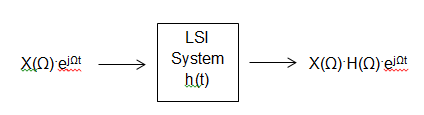
\includegraphics[width=0.7\textwidth]{fig1.png}
\caption{The Pulse Train with period $T_{s}$}
\end{figure}
Let's call this pulse train '$p(t)$' and let's try to find it's Fourier series expansion. We will use complex Fourier series, to write
\begin{align*}
C_{k}&=\frac{1}{T_{s}}\int\limits_{0}^{T_{s}} p(t) e^{-j\frac{2\pi}{T_{s}}kt}dt
\end{align*}
Where $C_{k}$ is the coefficient of the $k^{th}$ term in the Fourier series expansion, $T_{s}$ is the sampling period, and $j=\sqrt{-1}$.So we can write that expression (for nonzero $k$) as
\begin{align*}
C_{k}&=\frac{1}{T_{s}}\int\limits_{0}^{T_{s}} p(t) e^{-j\frac{2\pi}{T_{s}}kt}dt\\
         &=\frac{1}{T_{s}}\int\limits_{0}^{\Delta} e^{-j\frac{2\pi}{T_{s}}kt}dt\quad\text{as }p(t) \text{is nonzero, equal to one only in that region}\\
         &=\frac{1}{T_{s}}\left(\frac{e^{-j\frac{2\pi}{T_{s}}kt}}{-j\frac{2\pi}{T_{s}}k}\right)_{0}^{\Delta}\\
         &=\frac{e^{-j\frac{2\pi}{T_{s}}k\Delta}-1}{T_{s}\left(-j\frac{2\pi}{T_{s}}\right)k}\\
         &=\frac{1-e^{-j\frac{2\pi}{T_{s}}k\Delta}}{j2\pi k}\\
\end{align*}
We can simplify this as
\begin{align*}
C_{k}&=e^{-j\frac{2\pi}{T_{s}}k\frac{\Delta}{2}}\cdot \frac{\cancel{2j}\sin(\frac{\cancel{2}\pi}{T_{s}}k\frac{\Delta}{\cancel{2}})}{\cancel{2j}\pi k\frac{\Delta}{T_{s}}}\cdot\frac{\Delta}{T_{s}}\\
&=\frac{\Delta}{T_{s}}e^{-j\frac{2\pi}{T_{s}}k\frac{\Delta}{2}}\cdot\frac{\sin(\frac{\pi k \Delta}{T_{s}})}{\frac{\pi k \Delta}{T_{s}}}\\
&=\frac{\Delta}{T_{s}}e^{-j\frac{2\pi}{T_{s}}k\frac{\Delta}{2}}\cdot \text{sinc}\left(\frac{k\Delta}{T_{s}}\right)
\end{align*}
Where sinc function is given by
\begin{equation}
\text{sinc}(r)=\frac{\sin(\pi r)}{\pi r}\nonumber
\end{equation}
We can also scale these pulses so as to have unit area, by multiplying by $\frac{1}{\Delta}$, and it would just cancel out the delta in our expression, so we'd have 
\begin{equation}
C_{k}=\frac{1}{T_{s}}e^{-j\frac{2\pi}{T_{s}}k\frac{\Delta}{2}}\cdot \text{sinc}\left(\frac{k\Delta}{T_{s}}\right)\nonumber
\end{equation}
When $k=0$, we can show that $C_{0}$ is the limit of this expression as $k\rightarrow0$. We can also compute $C_{0}$ independently.\\
Let us plot the sinc function and see how it looks like:\\
\begin{figure}[htb]
\centering
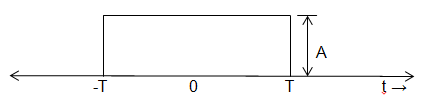
\includegraphics[width=0.3\textwidth]{fig2.png}
\caption{The 'sinc' function.}
\end{figure}
In ideal sampling, we had $\frac{\Delta}{T_{s}}$ very small, tending to zero. In that case we had all our samples taken very closely, around zero. Applying $\Delta\rightarrow0$ to the expression of $C_{k}$ (scaled), we have $C_{k}\approx\frac{1}{T_{s}}$ .i.e. all the $C_{k}$'s are same. However, if $\Delta\ne0$, we have the expression for $C_{k}$ as stated earlier, involving sinc function. We can write it as 
\begin{equation}
C_{k}=\gamma_0\text{sinc}\left(\frac{k\Delta}{T_{s}}\right)\nonumber
\end{equation}
Here $\gamma_0$ is a constant. Let's look at the Fourier series representation of $p(t)$:
\begin{figure}[htb]
\centering
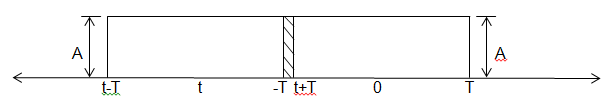
\includegraphics[width=0.3\textwidth]{fig3.png}
\caption{The sampled version of sinc($r$). $r$ is on the x-axis. Some of the $C_{i}$'s are labeled.}
\end{figure}
Note that the distance between two consecutive samples is $\frac{\Delta}{T_{s}}$. We can see that as $\Delta\rightarrow0$, we will have all our samples around zero. If $\frac{\Delta}{T_{s}}$ is quite large, after $C_{0}$, the second sample itself will be not from the main lobe. However, if we choose $\frac{\Delta}{T_{s}}$ to not be too large yet not too small, we would have first few samples from main lobe, and we can observe that they will be of decreasing magnitude.
\subsection{Sampling with the Pulse Train}
We already know that the Fourier series expansion of $p(t)$ is $\sum\limits_{k\in\mathbb{Z}}C_{k}e^{j\frac{2\pi}{T_{s}}kt}$, so multiplying it with $x(t)$, we'd have 
\begin{equation}
x(t)p(t)=\sum\limits_{k\in\mathbb{Z}}C_{k}x(t)e^{j\frac{2\pi}{T_{s}}kt}\nonumber
\end{equation}
Now let's take the Fourier transform of $x(t)p(t)$ which we have, assuming it exists. Note that, as Fourier transform is a linear transform, we can compute the Fourier transform of one term from the summation which we have, and add all such Fourier transforms. So we will compute Fourier transform of $x(t)e^{j\frac{2\pi}{T_{s}}kt}$.
\begin{align*}
\text{Fourier transform of }x(t)e^{j\frac{2\pi}{T_{s}}kt}&=\int\limits_{-\infty}^{+\infty}x(t)e^{j\frac{2\pi}{T_{s}}kt}e^{-j\Omega t}dt\\
&=\int\limits_{-\infty}^{+\infty}x(t)e^{-j\left(\Omega-\frac{2\pi}{T_{s}}k\right)}dt\\
\end{align*}
Suppose we have Fourier transform of $x(t)$ as $X(\Omega)$, then the Fourier transform of $x(t)e^{j\frac{2\pi}{T_{s}}kt}$ will be $X\left(\Omega-\frac{2\pi}{T_{s}}k\right)$, from the above equation. i.e. it is the Fourier transform of $x(t)$ namely $X(\Omega)$ shifted by $\frac{2\pi}{T_{s}}k$ forward. So we have 
\begin{align*}
&\text{Fourier transform of }x(t)e^{j\frac{2\pi}{T_{s}}kt}=X\left(\Omega-\frac{2\pi}{T_{s}}k\right)\\
\therefore\quad &\text{Fourier transform of }C_{k}x(t)e^{j\frac{2\pi}{T_{s}}kt}=C_{k}X\left(\Omega-\frac{2\pi}{T_{s}}k\right)\\
\therefore \quad&\text{Fourier transform of }\sum\limits_{k\in\mathbb{Z}}C_{k}x(t)e^{j\frac{2\pi}{T_{s}}kt}=\sum\limits_{k\in\mathbb{Z}}C_{k}X\left(\Omega-\frac{2\pi}{T_{s}}k\right)\\
\end{align*}
We can list down the procedure of finding the Fourier transform of $x(t)p(t)$ as follows:
\begin{enumerate}
\item Shift $X(\Omega)$ by $\frac{2\pi}{T_{s}k}$ forward, $\forall k\in\mathbb{Z}$.
\item Multiply this shifetd version of $X(\Omega)$ by $C_{k}$.
\item Add up all these shifted versions.
\end{enumerate}
\subsection{Graphical Representation of the Fourier Transform of the Sampled Signal}
We'll see how all of this looks graphically: Consider $x(t)$ to be bandlimited signal, as shown in the following image (magnitude of $X(\Omega)$ is shown in the image, and phase is considered to be zero for this signal everywhere:\\

\begin{figure}[htb]
\centering
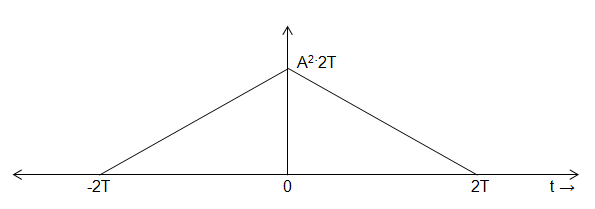
\includegraphics[width=0.35\textwidth]{fig4.png}
\caption{$X(\Omega)$}
\end{figure}

Note that this Fourier representation corresponds to a real and even signal $x(t)$.\\
We will first sample this signal 'disobeying' the Nyquist principle, i.e. by keeping $\frac{1}{T_{s}}\ngeq2\frac{\Omega_m}{2\pi}$. The first few $C_{}k$ values are seen in the following image:\\

\begin{figure}[htb]
\centering
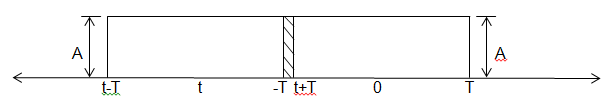
\includegraphics[width=0.3\textwidth]{fig3.png}
\end{figure}

Following the procedure given in the previous section, we obtain following spectrum for the sampled $x(t)$:\\

\begin{figure}[htb]
\centering
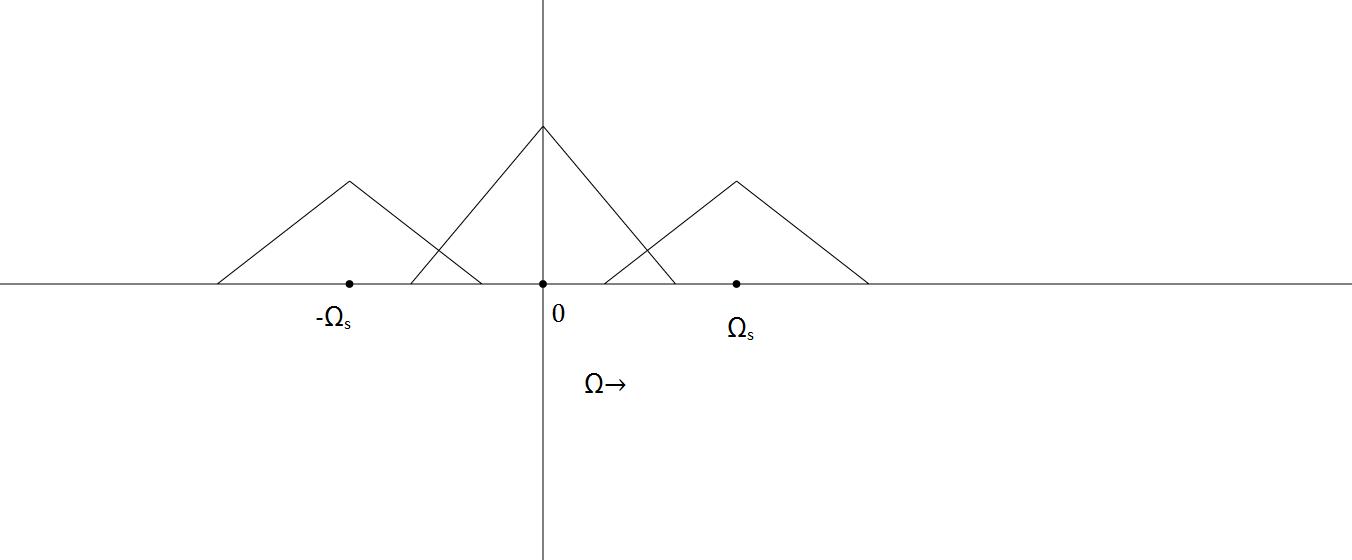
\includegraphics[width=0.7\textwidth]{fig5.png}
\caption{Fourier transform when we disobey Nyquist principle: shows overlaps.}
\end{figure}

One feature we can clearly see in this graph is that carbon copies of the original spectrum are overlapping: which we had already seen when we had sampled a similar signal with impulse train instead of pulse train (ideal sampling). However, there's one more remarkable thing we can see here: As the first few $C_k$'s are decreasing in magnitude, we observe that the 'strength' of the carbon copies is reducing, at least for first few $k$'s. So the carbon copies still overlap, but their strength is lower, or, the magnitude of overlap is less now, the region in which such overlap is occuring is closer to the original spectrum, if compared with the Fourier transform of the same signal, sampled using impulse train.\\
Now we will see what happens if we sample this signal 'obeying;' the Nyquist principle, i.e. $\frac{1}{T_{s}}\gg2\frac{\Omega_m}{2\pi}$. This time we obtain the spectrum of the sampled signal as following:\\

\begin{figure}[htb]
\centering
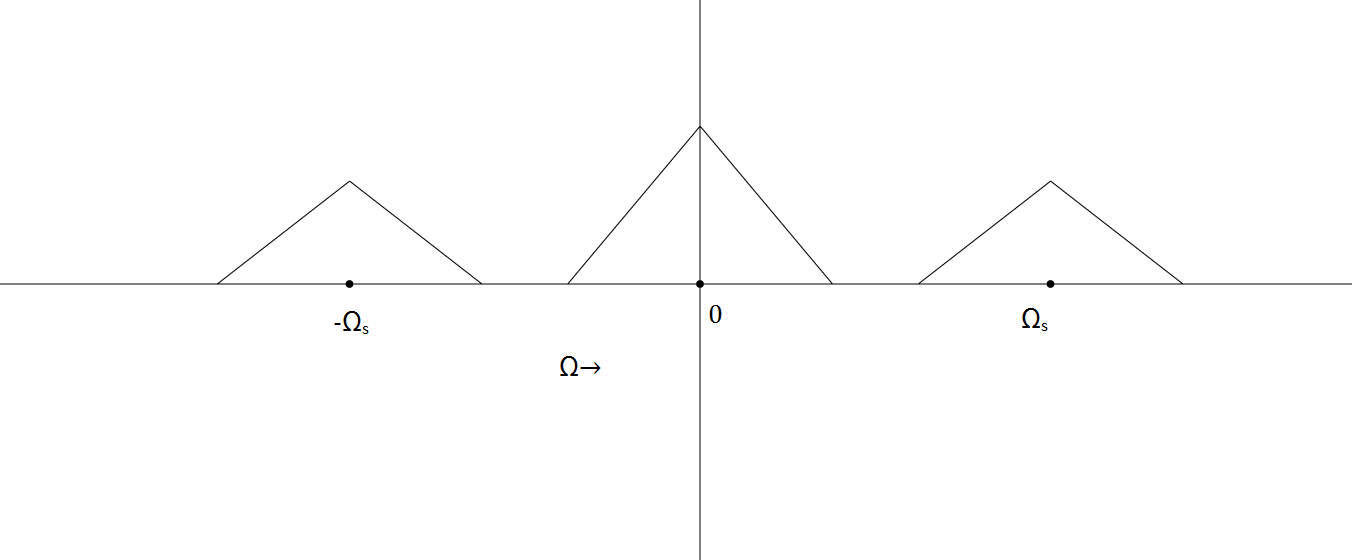
\includegraphics[width=0.7\textwidth]{fig6.png}
\caption{Fourier transform when we obey Nyquist principle: no overlap is seen.}
\end{figure}

Here, no overlap is seen between the original spectrum and any of its carbon copies, similar to when we had sampled using impulse train. But we can still see the magnitude of the first few carbon copies decreasing.\\
When reconstructing the signal back in this case, still need our spectrum to lie in the 'flat' region of the spectrum of the reconstructor (a simple practical example of which,  we have seen, is a simple $RC$- circuit). So pracically$\Omega_s$ needs to be much higher htan $\Omega_m$There is one more advantage of using pulse train instead of impulse train to sample a signal: for a practical reconstructor, it's spectrum desn't become zero directly after the flat region- it gradually tends towrd zero. So while reconstructing the signal, the higher-frequency carbon copies of the original spectrum aren't completely eliminated. Since we anyway have reducing magnitude for the carbon copies in the spectrum of the signal sampled using pulse train, we have lesser contribution from these high-frequency components than the reconstructed signal from the ideal sapmle of the signal.\\
We shall also give a name to these carbon copies: we will call them 'aliases' and this process 'aliasing' henceforth. Alias refers to the act of assuming a different identity. Here, original spectrum 'pretends' to be a spectrum around some $\Omega_s$. If these aliases interfere with each otherm it only causes confusion, Nyquist theorem essentially tells us htat we don't want aliasing.
